% Options for packages loaded elsewhere
\PassOptionsToPackage{unicode}{hyperref}
\PassOptionsToPackage{hyphens}{url}
%
\documentclass[
]{article}
\usepackage{amsmath,amssymb}
\usepackage{lmodern}
\usepackage{ifxetex,ifluatex}
\ifnum 0\ifxetex 1\fi\ifluatex 1\fi=0 % if pdftex
  \usepackage[T1]{fontenc}
  \usepackage[utf8]{inputenc}
  \usepackage{textcomp} % provide euro and other symbols
\else % if luatex or xetex
  \usepackage{unicode-math}
  \defaultfontfeatures{Scale=MatchLowercase}
  \defaultfontfeatures[\rmfamily]{Ligatures=TeX,Scale=1}
\fi
% Use upquote if available, for straight quotes in verbatim environments
\IfFileExists{upquote.sty}{\usepackage{upquote}}{}
\IfFileExists{microtype.sty}{% use microtype if available
  \usepackage[]{microtype}
  \UseMicrotypeSet[protrusion]{basicmath} % disable protrusion for tt fonts
}{}
\makeatletter
\@ifundefined{KOMAClassName}{% if non-KOMA class
  \IfFileExists{parskip.sty}{%
    \usepackage{parskip}
  }{% else
    \setlength{\parindent}{0pt}
    \setlength{\parskip}{6pt plus 2pt minus 1pt}}
}{% if KOMA class
  \KOMAoptions{parskip=half}}
\makeatother
\usepackage{xcolor}
\IfFileExists{xurl.sty}{\usepackage{xurl}}{} % add URL line breaks if available
\IfFileExists{bookmark.sty}{\usepackage{bookmark}}{\usepackage{hyperref}}
\hypersetup{
  hidelinks,
  pdfcreator={LaTeX via pandoc}}
\urlstyle{same} % disable monospaced font for URLs
\usepackage{graphicx}
\makeatletter
\def\maxwidth{\ifdim\Gin@nat@width>\linewidth\linewidth\else\Gin@nat@width\fi}
\def\maxheight{\ifdim\Gin@nat@height>\textheight\textheight\else\Gin@nat@height\fi}
\makeatother
% Scale images if necessary, so that they will not overflow the page
% margins by default, and it is still possible to overwrite the defaults
% using explicit options in \includegraphics[width, height, ...]{}
\setkeys{Gin}{width=\maxwidth,height=\maxheight,keepaspectratio}
% Set default figure placement to htbp
\makeatletter
\def\fps@figure{htbp}
\makeatother
\setlength{\emergencystretch}{3em} % prevent overfull lines
\providecommand{\tightlist}{%
  \setlength{\itemsep}{0pt}\setlength{\parskip}{0pt}}
\setcounter{secnumdepth}{-\maxdimen} % remove section numbering
\ifluatex
  \usepackage{selnolig}  % disable illegal ligatures
\fi

\author{}
\date{}

\begin{document}

\hypertarget{introduction}{%
\section{Introduction}\label{introduction}}

The intention of this documentation is to briefly explain a preliminary
study of the machine data and the potential they have when it comes to
detecting faults before they happen. The benefits of this application
are numerous and belong to the people who know closely the machine to
state it.\\
What is needed to understand the content below will be explained
throughout the document so that no previous knowledge is required to
understand the general idea. The results are pretty visual, so if you
get lost at some point, you will be able to keep following with ease.
Throughout the document, 4 fails will be shown:

\begin{itemize}
\item
  Fail 0: it will serve as a point of view of the early stages of the
  study and will introduce the graphics that will be seen in the other
  failures.
\item
  Fail 1, 2 and 3: it will serve as a point of view of the late stages
  of the study.
\end{itemize}

In the appendix there is more information about each failure and the
data used to study it.

\hypertarget{fail-0}{%
\section{Fail 0}\label{fail-0}}

In this document the same graphics will come out all the time, this
first example will serve to explain a little what they are and how they
can be interpreted. Let us remember that this is a real example that it
was done at the first steps of the study. As you will observe, at the
beginning not many results were achieved.\\
A series of tools have been used to obtain the data that will be
represented in the following graphics, some of the more important ones
are:

\begin{itemize}
\item
  \textbf{PCA}: principal component analysis, brings together different
  variables into one, in such a way that it maintains the properties and
  relations of the original variables. It is much easier to work with
  this data. \textbf{If you want to know more\ldots{}} it is a branch of
  the multivariate statistical analysis based on dimensionalty
  reduction. It makes a linear mapping of the data from the eigenvectors
  of the covariance matrix that correspond to the largest eigenvalues
  (main components).
\item
  \textbf{Mahalanobis distance}: measures the distance of a specific
  value from the other values in the dataset. In other words, it
  measures how anomalous or ``strange'' is a specific value. \textbf{If
  you want to know more\ldots{}} doing the standard deviation we could
  find how anomalous is a value with respect to the center of mass, but
  we would be assuming that the sample points are distributed in a
  spherical manner. When the distribution is non-spherical, for instance
  ellipsoidal, the probability of the test point depends not only on the
  center of mass, but also on the direction. The Mahalanobis distance
  keeps these things in mind.
\end{itemize}

Using the previous techniques (and more) the following graphic can be
obtained.\\
This example is one of the firsts analyzed. In this case it is a failure
that started on the 24.10.2016 and finished on the 27.10.2016. What is
analyzed is how the temperature of the compressor affected that failure.

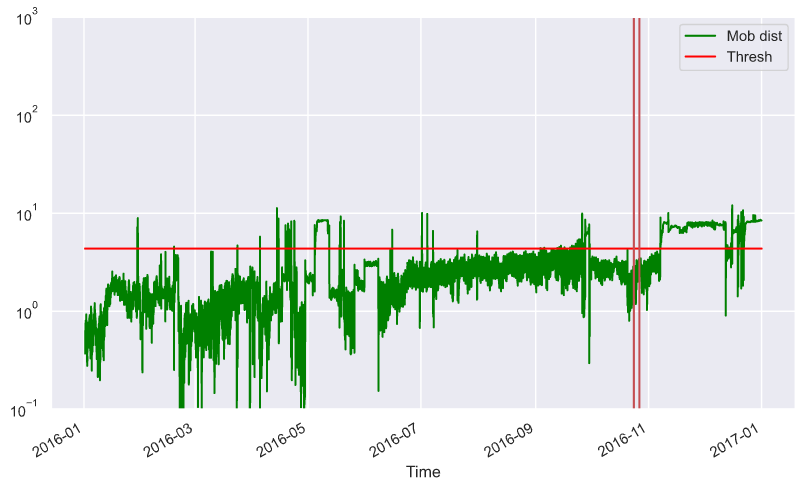
\includegraphics{relevant_graphs/4_4_AM.png} This is the first type of
graphic that we will see, in it is represented how anomalous each data
point is along all the data points in the dataset. The two vertical red
lines represent the beginning and the end of the failure respectively,
in this case 24.10.2016 to 27.10.2017. The horizontal red line is an
example of a threshold failure, where a notification could be sent.\\
As we can see, at the beginning of the study, without much knowledge
about the variables we did not get many results. There seems to be
nothing relevant in the graphic, the only thing that reflects is the
inability to detect failures.

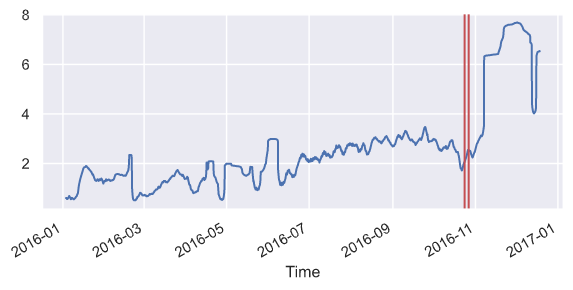
\includegraphics{relevant_graphs/4_4_T.png} This is the second type of
graphic that we will see, in it is represented the trend of the previous
graphic, that is, a more visual and intuitive way to see the general
path of the anomaly values. The failure beginning and end is represented
by the red vertical lines.\\
We can also appreciate that there does not appear to be any sufficiently
strange event before the failure, it doesn't look like we could have
detected anything.

\hypertarget{fail-1}{%
\section{Fail 1}\label{fail-1}}

In the previous section we were unable to detect anything. Now we will
see the study of three more failures, performed towards the end of the
study, where the knowledge about the variables was greater.\\
The fault we will see below started the 22.05.2017 and ended three days
later, the 25.05.2017. The data used to analyze the failure are two
variables that represent the axial displacement, and belong to the
compressor.

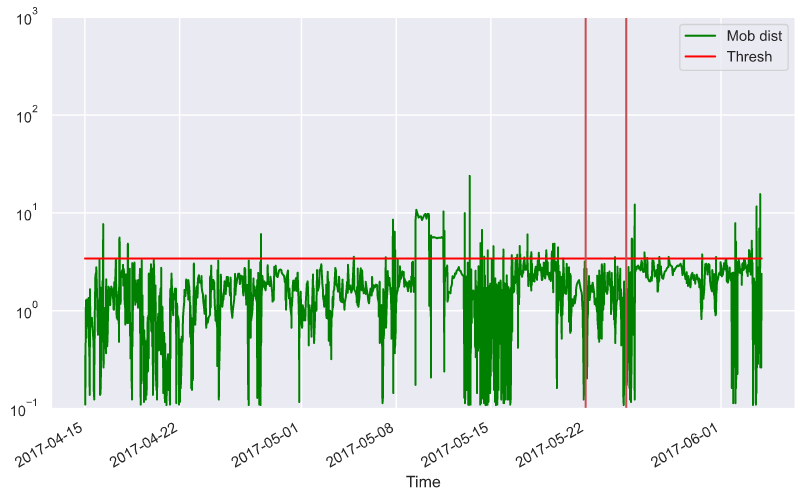
\includegraphics{relevant_graphs/6_1_AM.png} As we said, this graphic
reveals how abnormal each data point in the dataset is, apparently the
information represented in this graphic is difficult to see. The results
appear when we do the trend, in the following graphic.

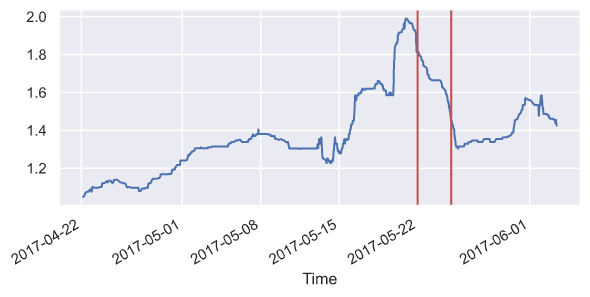
\includegraphics{relevant_graphs/6_1_T.png} Here is represented a
clearer and more visual way of what could be the deterioration of the
machine (or a part of it), culminating in its failure marked with the
first red line. The failure could have been detected over 10 days in
advance.

\hypertarget{fail-2}{%
\section{Fail 2}\label{fail-2}}

This failure starts on the 12.11.2018 and finishes on the 29.11.2018,
this time with data of temperature and vibration of the electric motor.
Same graphics, the result are self-explanatory.\\
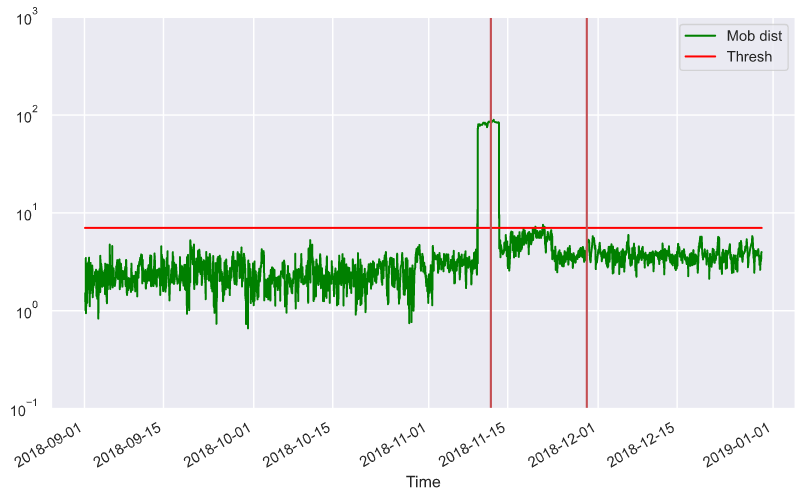
\includegraphics{relevant_graphs/7_3_AM.png}
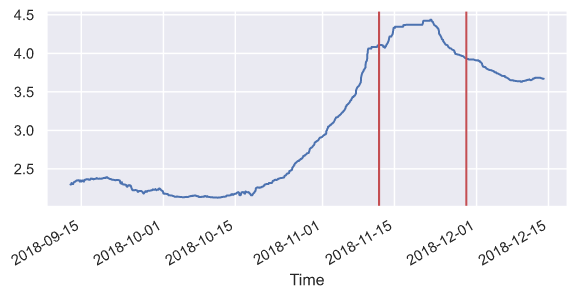
\includegraphics{relevant_graphs/7_3_T.png} Same conclusions as in the
previous section, a clear deterioration of the machine is seen,
foreseeable 10 days before.

\hypertarget{fail-3}{%
\section{Fail 3}\label{fail-3}}

The last failure that we will see occurred from the 20.07.2019 to the
31.07.2019. The data used belongs to the electric motor.\\
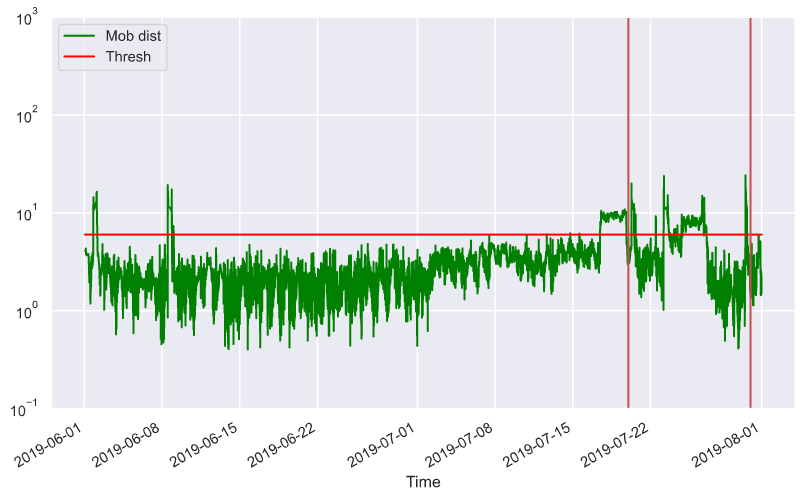
\includegraphics{relevant_graphs/8_3_AM.png}
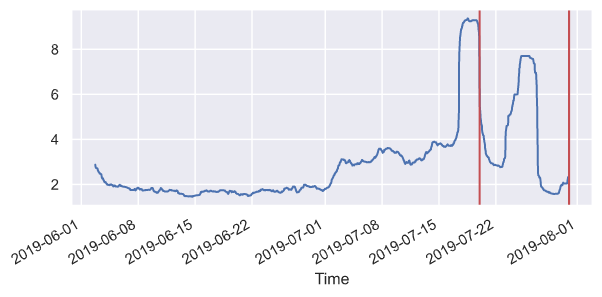
\includegraphics{relevant_graphs/8_3_T.png}

\hypertarget{precedence}{%
\section{Precedence}\label{precedence}}

This is not magic, so we can twitch and look closer to the data to
reveal more things. The potential is large if enough attention is paid,
and the ability to extract interesting information from it depends on
the creativity of the analyst, let's see the following example. We do
not only have the data in which we have observed the deterioration,
being able to select and reduce the number of possible culprits of the
failure, but we also have different ways of validate it. Look at the
following graphics:

\hypertarget{section}{%
\subsection{(1)}\label{section}}

\begin{figure}
\centering
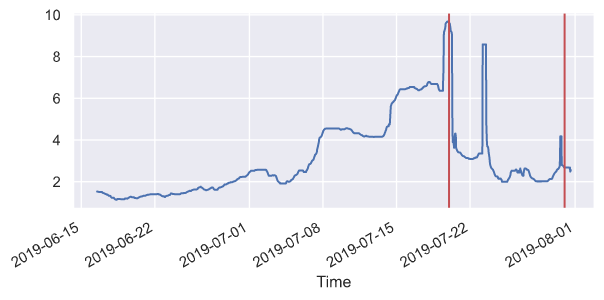
\includegraphics{relevant_graphs/prec_1.png}
\caption{Precedence 1}
\end{figure}

\hypertarget{section-1}{%
\subsection{(2)}\label{section-1}}

\begin{figure}
\centering
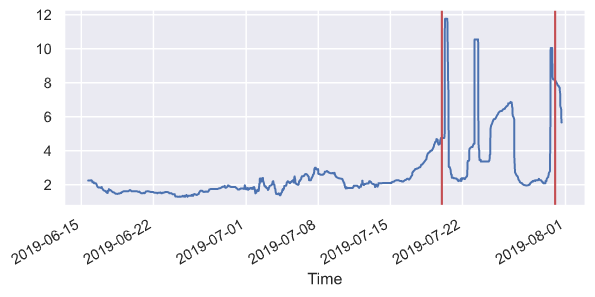
\includegraphics{relevant_graphs/prec_2.png}
\caption{Precedence 2}
\end{figure}

Both graphics are from the same fault, that of 20.07.2019 to 31.07.2019.
They are even from the part of the machine, the gearbox. The difference
is that the first is from the bearing 892B, and the second from the
bearing 891B. In the first graphic the deterioration is evident, and
most importantly, the peak occurs \textbf{before} the failure. Contrary
that in the second graphic, in which the deterioration is not very
obvious, and the peak occurs \textbf{after} the failure. This is a case
of precedence, which gives much information than it seems about the
failure.

\hypertarget{conclusions}{%
\section{Conclusions}\label{conclusions}}

This is not rocket science, it is only a preliminary study to show the
potential and the maneuverability that would come with more time and
better data.

\pagebreak

\hypertarget{annex}{%
\section{Annex}\label{annex}}

\hypertarget{annex-for-failure-0}{%
\subsection{Annex for failure 0}\label{annex-for-failure-0}}

Used variables: \textbf{HPI602, HPI605, HTI605}\\
Time of the failure: \textbf{24.10.2016 - 27.10.2016}\\
Training data graphic:\\
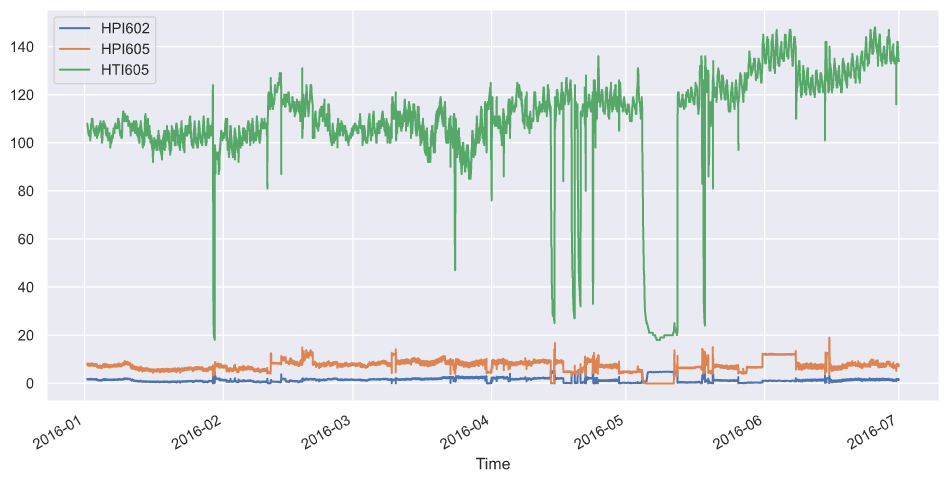
\includegraphics{relevant_graphs/train_fail0.png}

\hypertarget{annex-for-failure-1}{%
\subsection{Annex for failure 1}\label{annex-for-failure-1}}

Used variables: \textbf{HZI877B, HZI877C}\\
Time of the failure: \textbf{22.05.2017 - 25.05.2017}\\
Training data graphic:\\
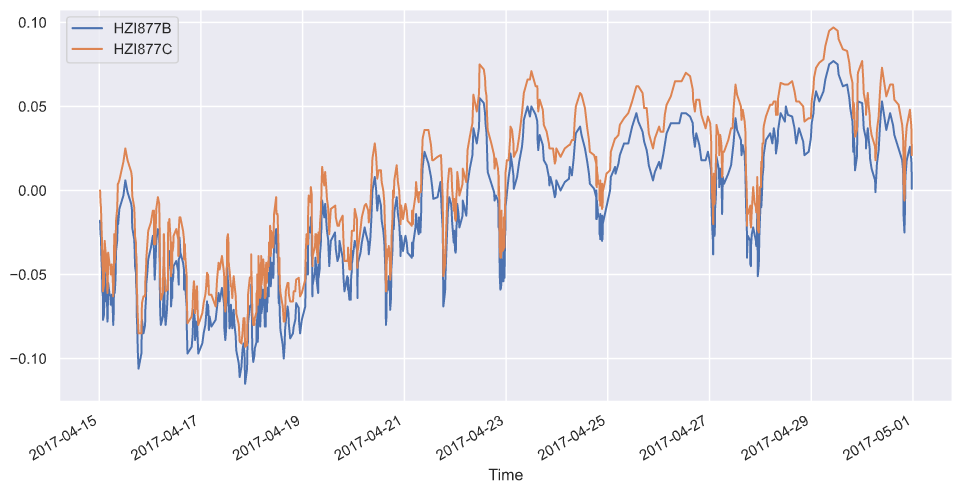
\includegraphics{relevant_graphs/train_fail1.png}

\hypertarget{annex-for-failure-2}{%
\subsection{Annex for failure 2}\label{annex-for-failure-2}}

Used variables: \textbf{HTI880A, HTI879B, HTI883A, HVI877X, HVI877Y,
HVI878Y}\\
Time of the failure: \textbf{12.11.2018 - 29.11.2018}\\
Training data graphic:\\
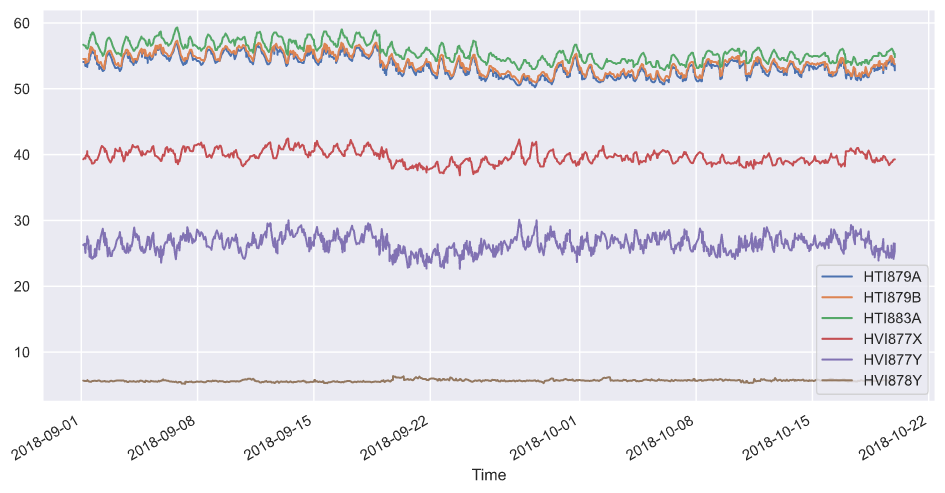
\includegraphics{relevant_graphs/train_fail2.png}

\hypertarget{annex-for-failure-3}{%
\subsection{Annex for failure 3}\label{annex-for-failure-3}}

Used variables: \textbf{HTI879A, HTI879B, HTI883A, HVI877X, HVI877Y,
HVI878Y}\\
Time of the failure: \textbf{20.07.2019 - 31.07.2019}\\
Training data graphic:\\
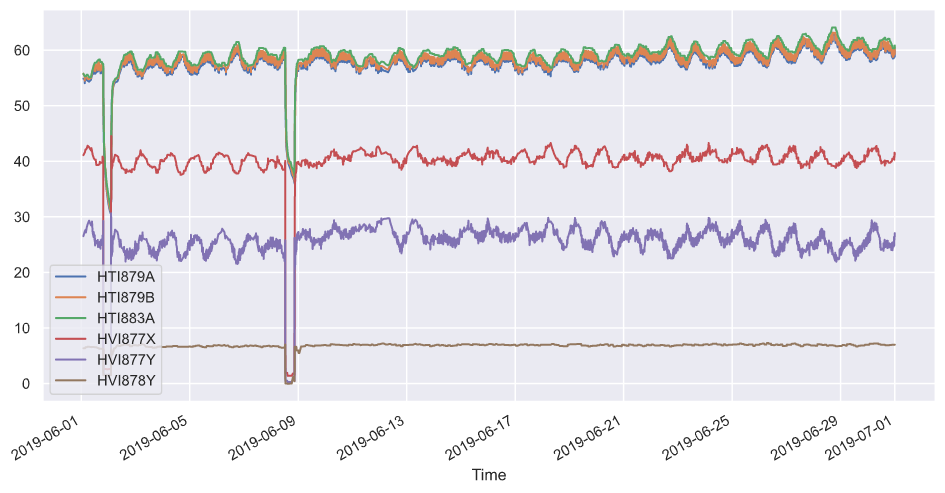
\includegraphics{relevant_graphs/train_fail3.png}

\end{document}
